
\chapter{Introduzione}


\section{TCP/Ip e modello a strati}

% https://en.wikipedia.org/wiki/Internet_protocol_suite
% https://it.wikipedia.org/wiki/Modello_OSI
% https://datatracker.ietf.org/doc/html/rfc1122
% https://datatracker.ietf.org/doc/html/rfc791
% https://datatracker.ietf.org/doc/html/rfc791#section-2.1
% https://datatracker.ietf.org/doc/html/rfc791#section-2.2

% to be removed
\subsection{cos'e' internet}

%%% \cite https://datatracker.ietf.org/doc/html/rfc1122#section-1
% An Internet communication system consists of interconnected packet networks supporting communication among host computers using the Internet protocols.  The networks are interconnected using packet-switching computers called "gateways" or "IP routers" by the Internet community, and "Intermediate Systems" by the OSI world [INTRO:13].
%%%

L'architettura che determina il funzionamento di Internet si basa su un modello a strati, in cui ogni strato e' indipendente da quelli sottostanti.

\subsection{Internet Protocol Suite}

%%  Internet Protocol Suite
%%
%%    To communicate using the Internet system, a host must implement
%%    the layered set of protocols comprising the Internet protocol
%%    suite.  A host typically must implement at least one protocol
%%    from each layer.

Per comunicare su Internet, gli Host devono implementare un set di protocolli che costituiscono l'\it{Internet protocol suite} \cite{RFC_1122}. I protocolli si suddividono in strati logici che li raggruppano in 4 categorie, ogni Host deve implementare almeno un protocollo per ogni strato.

\begin{figure}[H]
    \centering
    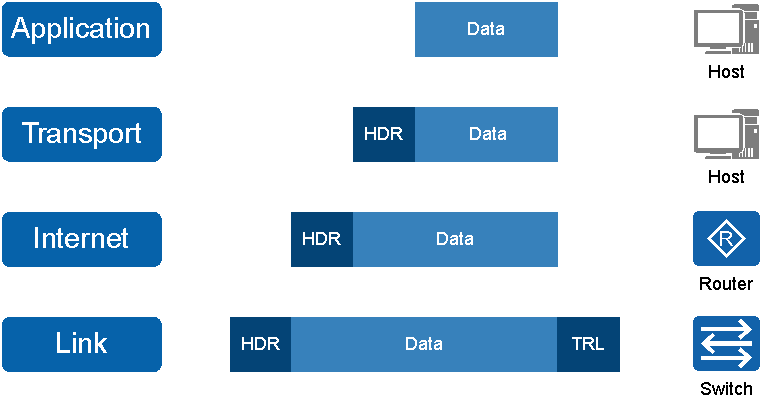
\includegraphics[width=0.8\textwidth]{immagini/diag2-modello_a_strati}
    \caption{Rappresentazione degli strati del modello TCP/Ip con relativo incapsulamento e dispositivo di dominio}
    \label{fig:modello-a-strati}
\end{figure}



%%    The protocol layers used in the Internet architecture are as
%%    follows [INTRO:4]:

\begin{enumerate} % \cite https://datatracker.ietf.org/doc/html/rfc1122#section-1
    \item[4.] \textbf{Application Layer}: Il livello applicazione e' il layer piu' alto dell'\it{Internet protocol suite}, i protocolli di questo livello si suddividono in protocolli utente e di supporto. \newline
    I protocolli utente espongono un servizio direttamente all'utente finale, alcuni esempi sono: \href{https://en.wikipedia.org/wiki/Hypertext_Transfer_Protocol}{http}, \href{https://en.wikipedia.org/wiki/File_Transfer_Protocol}{ftp}, \href{https://en.wikipedia.org/wiki/Secure_Shell}{ssh}, etc. \newline
    I protocolli di supporto forniscono alcune fuinzionalita' di supporto per il funzionamento della rete, alcuni esempi sono: \href{https://en.wikipedia.org/wiki/Domain_Name_System}{DNS}, \href{https://en.wikipedia.org/wiki/Simple_Network_Management_Protocol}{SNMP} etc.

%%        The application layer is the top layer of the Internet
%%        protocol suite.  The Internet suite does not further
%%        subdivide the application layer, although some of the
%%        Internet application layer protocols do contain some
%%        internal sub-layering.  The application layer of the
%%        Internet suite essentially combines the functions of the
%%        top two layers -- Presentation and Application -- of the
%%        OSI reference model.
%%
%%        We distinguish two categories of application layer
%%        protocols:  user protocols that provide service directly
%%        to users, and support protocols that provide common system
%%        functions.  Requirements for user and support protocols
%%        will be found in the companion RFC [INTRO:1].
%%
%%        The most common Internet user protocols are:
%%
%%        o  Telnet (remote login)
%%        o  FTP    (file transfer)
%%        o  SMTP   (electronic mail delivery)
%%
%%        There are a number of other standardized user protocols
%%        [INTRO:4] and many private user protocols.
%%
%%        Support protocols, used for host name mapping, booting,
%%        and management, include SNMP, BOOTP, RARP, and the Domain
%%        Name System (DNS) protocols.


    \item[3.] \textbf{Transport Layer}: Il livello di trasporto fornisce una comunicazione end-to-end tra per le applicazioni, infatti in generale il campo data del livello di trasporto non viene letto da nessuno se non l'applicazione di sorgente e destinazione. \newline
    I protocolli principali di questo livello sono TCP e UDP: il \href{https://en.wikipedia.org/wiki/Transmission_Control_Protocol}{TCP} e' connection-oriented e fornisce alta affidabilita'; mentre l'\href{https://en.wikipedia.org/wiki/User_Datagram_Protocol}{UDP} e' connection-less, quindi ogni inaffidabilità della rete deve essere gestita a livello applicazione.
    
%%        The transport layer provides end-to-end communication
%%        services for applications.  There are two primary
%%        transport layer protocols at present:
%%
%%        o Transmission Control Protocol (TCP)
%%        o User Datagram Protocol (UDP)
%%
%%        TCP is a reliable connection-oriented transport service
%%        that provides end-to-end reliability, resequencing, and
%%        flow control.  UDP is a connectionless ("datagram")
%%        transport service.
%%
%%        Other transport protocols have been developed by the
%%        research community, and the set of official Internet
%%        transport protocols may be expanded in the future.
%%
%%        Transport layer protocols are discussed in Chapter 4.

    % TODO da rivedere
    \item[2.] \textbf{Internet Layer}: Tutti i protocolli di trasporto usano il protocollo Internet (IP) per portare i dati dall'host sorgente alla destinazione. Al contrario dei protocolli di livello trasporto il protocollo IP non e' end-to-end, quindi e' intrinsecamente di tipo connection-less, non fornisce quindi nessuna garanzia che il pacchetto arrivi a destinazione, o arrivi danneggiato o duplicato. I layer sopra al livello IP sono responsabili di mantenere l'affidabilita' dei servizi quando essa e' richiesta. \newline 
    Di questo layer fanno parte i protocolli \href{https://en.wikipedia.org/wiki/Internet_Protocol}{IP}, \href{https://en.wikipedia.org/wiki/Internet_Control_Message_Protocol}{ICMP}, etc.
    
%%        All Internet transport protocols use the Internet Protocol
%%        (IP) to carry data from source host to destination host.
%%        IP is a connectionless or datagram internetwork service,
%%        providing no end-to-end delivery guarantees. Thus, IP
%%        datagrams may arrive at the destination host damaged,
%%        duplicated, out of order, or not at all.  The layers above
%%        IP are responsible for reliable delivery service when it
%%        is required.  The IP protocol includes provision for
%%        addressing, type-of-service specification, fragmentation
%%        and reassembly, and security information.
%%
%%        The datagram or connectionless nature of the IP protocol
%%        is a fundamental and characteristic feature of the
%%        Internet architecture.  Internet IP was the model for the
%%        OSI Connectionless Network Protocol [INTRO:12].
%%
%%        ICMP is a control protocol that is considered to be an
%%        integral part of IP, although it is architecturally
%%        layered upon IP, i.e., it uses IP to carry its data end-
%%        to-end just as a transport protocol like TCP or UDP does.
%%        ICMP provides error reporting, congestion reporting, and
%%        first-hop gateway redirection.
%%
%%        IGMP is an Internet layer protocol used for establishing
%%        dynamic host groups for IP multicasting.
%%
%%        The Internet layer protocols IP, ICMP, and IGMP are
%%        discussed in Chapter 3.

    % TODO da rivedere
    \item[1.] \textbf{Link Layer}: E' il layer piu' vicino al mezzo fisico su cui viaggiano i dati, ogni host deve implementare il protocollo usato per la specifica interfaccia che usa. Ad esempio un'host con un'interfaccia Ethernet deve implementare i protocolli.. ?
    
%%        To communicate on its directly-connected network, a host
%%        must implement the communication protocol used to
%%        interface to that network.  We call this a link layer or
%%        media-access layer protocol.
%%
%%        There is a wide variety of link layer protocols,
%%        corresponding to the many different types of networks.
%%        See Chapter 2.

\end{enumerate}

Possiamo vedere a cosa corrisponde in pratica con una cattura di un pacchetto eseguita con \it{Wireshark}:

\begin{bashcode}{Wireshark}{code:tls-wireshark}
1 > Frame 43408: 93 bytes on wire (744 bits), 93 bytes captured (744 bits) on interface wlp5s0, id 0
1 > Ethernet II, Src: IntelCor_eb:91:5f (cc:d9:ac:eb:91:5f), Dst: HuaweiDe_27:a9:24 (0c:e4:a0:27:a9:24)
2 > Internet Protocol Version 4, Src: 192.168.8.119, Dst: 142.250.180.174
3 > Transmission Control Protocol, Src Port: 36354, Dst Port: 443, Seq: 36720, Ack: 13639, Len: 39
4 > Transport Layer Security
     > TLSv1.3 Record Layer: Application Data Protocol: http-over-tls
             Opaque Type: Application Data (23)
             Version: TLS 1.2 (0x0303)
             Length: 34
             Encrypted Application Data: 389bf9516cce567d0d90ef62ba2a87376091fedb7f66f3b9e60e45a39376b1ae667a
             [Application Data Protocol: http-over-tls]
\end{bashcode}

\subsection{Incapsulamento}

Ogni protocollo di ogni layer aggiunge un header e un trailer, come si vede in fig. \ref{fig:modello-a-strati}.
Ad esempio analizzando la cattura in Wireshark, code. \ref{code:tls-wireshark}, si puo' vedere lo stack dei protocolli e i loro relativi header:

\begin{itemize}
    \item \textbf{Ethernet II}: Aggiunge 14 bytes di header e 4 bytes di trailer \cite{ethernet-ii}.
    \item \textbf{Internet Protocol Version 4}: Aggiunge un minimo di 20 bytes di header \cite{RFC_0791}
    \item \textbf{Transmission Control Protocol}: Aggiunge un minimo di 20 bytes di header \cite{RFC_0793}
    \item \textbf{Transport Layer Security}: \cite{RFC_8446} % TODO 
\end{itemize}

Si vede come sono stati aggiunti complessivamente un minimo di 58 bytes di hoverhead dovuti ai protocolli.

\section{Openvpn}

% https://wiki.wireshark.org/OpenVPN
% https://build.openvpn.net/doxygen/network_protocol.html

%%   OpenVPN [OpenVPN] is a commonly used protocol designed as an
%%   alternative to IPsec.  A major goal of this protocol is to provide a
%%   VPN that is simple to configure and works over a variety of
%%   transports.  OpenVPN encapsulates either IP packets or Ethernet
%%   frames within a secure tunnel and can run over either UDP or TCP.
%%   For key establishment, OpenVPN can either use TLS as a handshake
%%   protocol or use pre-shared keys.

OpenVPN e' un applicativo opensource che permette di instaurare una connessione VPN tra computer. Fa uso di protocolli di crittografia che garantiscono che la connessione sia privata e sicura.
Al contrario di altri protocolli VPN, come % TODO vedi da slide huawei nella parte delle vpn

e' di livello applicazione e va incapsulato in udp o tcp,

vediamo una cattura di wireshark:

\begin{bashcode}{Wireshark}{}
> Frame 90: 82 bytes on wire (656 bits), 82 bytes captured (656 bits) on interface br-08876ccdf1f5, id 0
> Ethernet II, Src: 02:42:0a:00:04:03 (02:42:0a:00:04:03), Dst: 02:42:0a:00:04:02 (02:42:0a:00:04:02)
> Internet Protocol Version 4, Src: 10.0.4.3, Dst: 10.0.4.2
> User Datagram Protocol, Src Port: 47007, Dst Port: 1194
> OpenVPN Protocol
        Type: 0x48 [opcode/key_id]
        Peer ID: 0
        Data (36 bytes)
            Data: 00000019a366196eb2aca181df226faf8514ab73f524f7ef335d55fc57322d032a2095e4
\end{bashcode}

% TODO do not like -> https://it.wikipedia.org/wiki/OpenVPN#Rete
All'interno del campo data del pacchetto openvpn vi e', criptato, un pacchetto IP o addirittura anche un pacchetto ethernet.

Per la cifratura si serve della libreria OpenSSL, ne supporta quindi tutti i protocolli di cifratura. Ha inoltre ulteriori estensioni alla sicurezza come l'utilizzo dell'autenticazione di pacchetto HMAC.

% https://en.wikipedia.org/wiki/Pre-shared_key

\section{Openwrt}

OpenWRT e' un sistema operativo per sistemi enbedded, e' principalmente usato nei router. E' basato su kernel linux, con specifica attenzione dell'ottimizazione del sistema per fare in modo che possa eseguirsi su sistemi con risorse estremamente ridotte.
Al contrario di altri sistemi operativi per dispositivi embedding, OpenWRT presenta un filesystem con permessi di scrittura, cio' permette all'utente di accedervi e modificare a runtime le funzionalita' del dispositivo.

Comprende una shell linux comprensiva delle funzionalita' piu' comuni, compreso il suo gestore pacchetti opkg.

OpenWRT puo' essere configurato sia tramite shell che tramite interfaccia web (LuCI).

% TODO move the openwrt shell banner e gli screen di luci

